% =============================================================================
% Guía de Laboratorio (combinada) — IA y Visión por Computadora
% PUCP · Ing. Mecatrónica · 1MTR56 — Automatización Industrial Inteligente B
% Parte 1: CNN (fundamentos)   ·   Parte 2: Transfer Learning + Beckhoff
% Nota del laboratorio = Parte 1 (/10) + Parte 2 (/10) = /20
% =============================================================================
% =============================================================================
% Plantilla LaTeX para guías del curso 1MTR56 — Automatización Industrial
% Inteligente B (PUCP, Ing. Mecatrónica).
%
% Replica el estilo del documento de referencia:
%   docs/archivo/1MTR56 - Laboratorio 1 - IPC Beckhoff.pdf
%
% Compilar con: xelatex (necesario para fontspec / fuentes del sistema)
% =============================================================================
\documentclass[12pt,a4paper]{article}

% ---------- Tipografía ----------
\usepackage{fontspec}
\usepackage{iftex}
% Prefiere Liberation Sans (Arial libre); si no está, DejaVu Sans.
\IfFontExistsTF{Liberation Sans}{%
  \setmainfont{Liberation Sans}[Ligatures=TeX, Scale=1.0]%
  \setmonofont{Liberation Mono}[Scale=0.92]%
}{%
  \setmainfont{DejaVu Sans}[Ligatures=TeX, Scale=0.95]%
  \setmonofont{DejaVu Sans Mono}[Scale=0.90]%
}
\usepackage{microtype}

% ---------- Idioma ----------
\usepackage{polyglossia}
\setdefaultlanguage{spanish}

% Macro para insertar el índice con el título correcto sin importar el
% comportamiento de polyglossia/babel sobre \contentsname.
\newcommand{\indicepucp}{%
  \renewcommand{\contentsname}{Tabla de contenido}%
  \tableofcontents%
}

% ---------- Geometría de página ----------
\usepackage[a4paper,
            top=3cm,
            bottom=3cm,
            left=2.5cm,
            right=2.5cm,
            headheight=14pt,
            headsep=1cm,
            footskip=1.2cm]{geometry}

% ---------- Header / footer ----------
\usepackage{fancyhdr}
\pagestyle{fancy}
\fancyhf{}
\fancyhead[L]{\footnotesize PONTIFICIA UNIVERSIDAD CATÓLICA DEL PERÚ}
\fancyhead[R]{\footnotesize INGENIERÍA MECATRÓNICA}
\fancyfoot[L]{\footnotesize 1MTR56 AUTOMATIZACIÓN INDUSTRIAL INTELIGENTE B}
\fancyfoot[R]{\footnotesize \thepage}
\renewcommand{\headrulewidth}{0pt}
\renewcommand{\footrulewidth}{0pt}

% Estilo de portada: sin header/footer
\fancypagestyle{portada}{%
  \fancyhf{}\renewcommand{\headrulewidth}{0pt}\renewcommand{\footrulewidth}{0pt}
}

% ---------- Numeración de secciones ----------
\usepackage{titlesec}
\titleformat{\section}{\Large\bfseries}{\thesection}{1em}{}
\titleformat{\subsection}{\large\bfseries}{\thesubsection}{1em}{}
\titleformat{\subsubsection}{\normalsize\bfseries}{\thesubsubsection}{1em}{}
\titlespacing*{\section}{0pt}{18pt}{8pt}
\titlespacing*{\subsection}{0pt}{14pt}{6pt}
\titlespacing*{\subsubsection}{0pt}{10pt}{4pt}

% ---------- Tabla de contenido con dotted leaders ----------
\usepackage{tocloft}
\renewcommand{\cftsecleader}{\cftdotfill{\cftdotsep}}
\renewcommand{\cftsubsecleader}{\cftdotfill{\cftdotsep}}
\setlength{\cftbeforesecskip}{4pt}
\renewcommand{\contentsname}{Tabla de contenido}

% ---------- Figuras y tablas ----------
\usepackage{graphicx}
\usepackage{caption}
\captionsetup{font=small,labelfont=bf,labelsep=period,justification=centering}
\usepackage{booktabs}
\usepackage{array}
\usepackage{tabularx}

% ---------- TikZ para diagramas vectoriales nativos ----------
\usepackage{tikz}
\usetikzlibrary{positioning, arrows.meta, shapes.geometric, fit, backgrounds, calc}
\tikzset{
  pucpbox/.style={
    rectangle, rounded corners=3pt,
    draw=PUCPblue, line width=0.8pt,
    fill=white,
    minimum height=1.3cm, minimum width=2.6cm,
    align=center,
    font=\small
  },
  pucpboxfilled/.style={
    pucpbox,
    fill=PUCPblue, text=white,
    font=\small\bfseries
  },
  pucparrow/.style={
    -{Stealth[length=2.5mm,width=2mm]},
    line width=0.7pt, draw=black!70
  }
}

% ---------- Colores institucionales (uso mínimo) ----------
\usepackage{xcolor}
\definecolor{PUCPblue}{HTML}{1F3864}

% ---------- Hipervínculos ----------
\usepackage[hidelinks,bookmarks=true,bookmarksopen=true]{hyperref}

% ---------- Listas ----------
\usepackage{enumitem}
\setlist{topsep=6pt,itemsep=4pt,parsep=0pt,leftmargin=18pt}

% ---------- Espaciado entre párrafos ----------
\usepackage{parskip}
\setlength{\parskip}{6pt plus 1pt minus 0pt}
\setlength{\parindent}{0pt}

% ---------- Código fuente ----------
\usepackage{listings}
\lstdefinestyle{pucp}{
  basicstyle=\ttfamily\footnotesize,
  keywordstyle=\bfseries\color{PUCPblue},
  commentstyle=\color{gray}\itshape,
  stringstyle=\color{black!70},
  showstringspaces=false,
  breaklines=true,
  frame=single,
  rulecolor=\color{black!30},
  framerule=0.4pt,
  xleftmargin=10pt,
  xrightmargin=10pt,
  aboveskip=10pt,
  belowskip=10pt,
}
\lstset{style=pucp}

% Evitar desbordes de margen con tokens largos (rutas, \texttt)
\setlength{\emergencystretch}{3em}
\sloppy
% Renombrar "Listing" → "Script" en captions de lstlisting
\renewcommand{\lstlistingname}{Script}

% =============================================================================
% Variables del documento (sobreescribibles)
% =============================================================================
\newcommand{\labtitulo}{LABORATORIO}
\newcommand{\labnumero}{X}
\newcommand{\labsubtitulo}{Título del laboratorio}

% =============================================================================
% Comando: \portadapucp{<num>}{<subtitulo>}
%
% Diseño basado en docs/archivo/1MTR56 - Laboratorio 1 - IPC Beckhoff.pdf
% pero con proporciones revisadas (logo dominante, mayor aire entre bloques,
% jerarquía tipográfica de tres niveles).
% =============================================================================
\newcommand{\portadapucp}[2]{%
  \thispagestyle{portada}
  \begin{titlepage}
  \begin{center}
    \vspace*{0.6cm}

    % ====================================================================
    % BLOQUE 1 — Identidad institucional (jerarquía: 18pt → 14pt → 14pt)
    % ====================================================================
    {\fontsize{18}{22}\selectfont\bfseries PONTIFICIA UNIVERSIDAD CATÓLICA DEL PERÚ}

    \vspace{1.2cm}

    {\fontsize{14}{18}\selectfont FACULTAD DE CIENCIAS E INGENIERÍA}\\[0.55cm]
    {\fontsize{14}{18}\selectfont INGENIERÍA MECATRÓNICA}

    \vfill

    % ====================================================================
    % BLOQUE 2 — Logo institucional dominante
    % ====================================================================
    
\includegraphics[width=0.80\textwidth]{../docs/assets/branding/pucp_logo.jpg}

    \vfill

    % ====================================================================
    % BLOQUE 3 — Título del laboratorio (centerpiece del documento)
    % ====================================================================
    \rule{0.65\textwidth}{0.5pt}\\[0.8cm]
    {\fontsize{16}{20}\selectfont\bfseries LABORATORIO #1: #2}\\[0.6cm]
    \rule{0.65\textwidth}{0.5pt}

    \vfill

    % ====================================================================
    % BLOQUE 4 — Identificación del curso
    % ====================================================================
    {\fontsize{14}{18}\selectfont\bfseries 1MTR56}\\[0.5cm]
    {\fontsize{14}{18}\selectfont\bfseries AUTOMATIZACIÓN INDUSTRIAL INTELIGENTE B}

    \vfill

    % ====================================================================
    % BLOQUE 5 — Ciclo académico (footer simbólico)
    % ====================================================================
    {\fontsize{13}{16}\selectfont 2026 -- 1}

    \vspace{0.6cm}
  \end{center}
  \end{titlepage}
}


\renewcommand{\partname}{Parte}
\renewcommand{\thepart}{\arabic{part}}

\begin{document}

\portadapucp{}{INTELIGENCIA ARTIFICIAL Y VISIÓN POR COMPUTADORA}

\indicepucp
\thispagestyle{fancy}
\newpage

\clearpage
\part{Inteligencia Artificial: Redes Neuronales Convolucionales}
\section{Introducción}

Esta guía introduce los fundamentos de la \emph{visión por computadora} basada en
aprendizaje profundo y los aplica a un problema de clasificación de imágenes con
\emph{redes neuronales convolucionales} (CNN). Constituye la \textbf{Parte~1} del
laboratorio: se entrena una CNN \emph{desde cero}; la Parte~2 introducirá el
aprendizaje por transferencia sobre el mismo dominio.

\textbf{Materiales.} Python 3.10 con el entorno del laboratorio; el dataset de
botellas provisto en \texttt{data/botellas/}; y los tres notebooks de la carpeta
\texttt{parte1\_ia/} (Notebook~1 a Notebook~3). Cada notebook explica su código en
detalle; esta guía es la referencia teórica y describe \emph{qué} se hace y
\emph{cuánto} aporta a la evaluación.

\section{Preparación del entorno en VS Code}

El único requisito delicado es usar un entorno virtual con la \textbf{versión correcta de
Python} (3.10 o 3.11): con otra versión, TensorFlow no se instala correctamente.

\begin{enumerate}
  \item Abrir la carpeta del proyecto en \textbf{Visual Studio Code}.
  \item \emph{Command Palette} (\texttt{Ctrl+Shift+P}) $\rightarrow$
        \texttt{Python: Create Environment} $\rightarrow$ \texttt{Venv} $\rightarrow$ elegir
        un intérprete \textbf{Python 3.10} o \textbf{3.11}. Cuando VS Code lo solicite,
        marcar \texttt{requirements.txt} para que instale las dependencias en ese entorno.
  \item En cada notebook, \texttt{Select Kernel} (arriba a la derecha) y elegir el entorno
        \texttt{.venv} recién creado.
\end{enumerate}

Con el entorno correcto seleccionado, las celdas de \texttt{import} de los notebooks
funcionan directamente (las dependencias ya quedaron instaladas al crear el entorno). Para
confirmar la versión:

\begin{lstlisting}[language=Python]
import sys, tensorflow as tf
print(sys.version)        # 3.10.x o 3.11.x
print(tf.__version__)     # 2.20.0
\end{lstlisting}

\section{Redes neuronales convolucionales}

Una CNN aprende a extraer características visuales directamente de los píxeles, sin
ingeniería manual de \emph{features}. Se compone de tres tipos de capas
(Figura~\ref{fig:cnn}):

\begin{itemize}
  \item \textbf{Convolución} (\texttt{Conv2D}): aplica filtros que se deslizan sobre la
        imagen y detectan patrones locales ---bordes, texturas, formas---. Los filtros
        se aprenden durante el entrenamiento (Figura~\ref{fig:conv}).
  \item \textbf{Pooling} (\texttt{MaxPooling2D}): reduce la resolución conservando la
        información dominante, lo que aporta robustez y disminuye el cómputo
        (Figura~\ref{fig:pool}).
  \item \textbf{Capas densas} (\texttt{Dense}): combinan las características extraídas; la
        capa de salida usa \emph{softmax} para producir una probabilidad por clase.
\end{itemize}

La función de activación \emph{ReLU} introduce la no linealidad entre capas; sin ella la
red colapsaría a una única transformación lineal (Figura~\ref{fig:act}).

\begin{figure}[h]
\centering
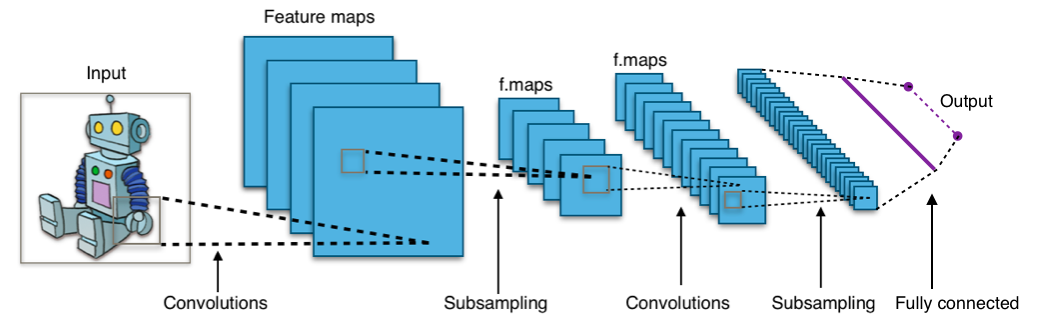
\includegraphics[width=0.92\textwidth]{../docs/assets/g1/typical_cnn_wikimedia.png}
\caption{Arquitectura típica de una CNN: bloques de convolución y pooling extraen características de complejidad creciente; las capas densas producen la clasificación. Fuente: Wikimedia Commons (CC BY-SA).}
\label{fig:cnn}
\end{figure}

\begin{figure}[h]
\centering
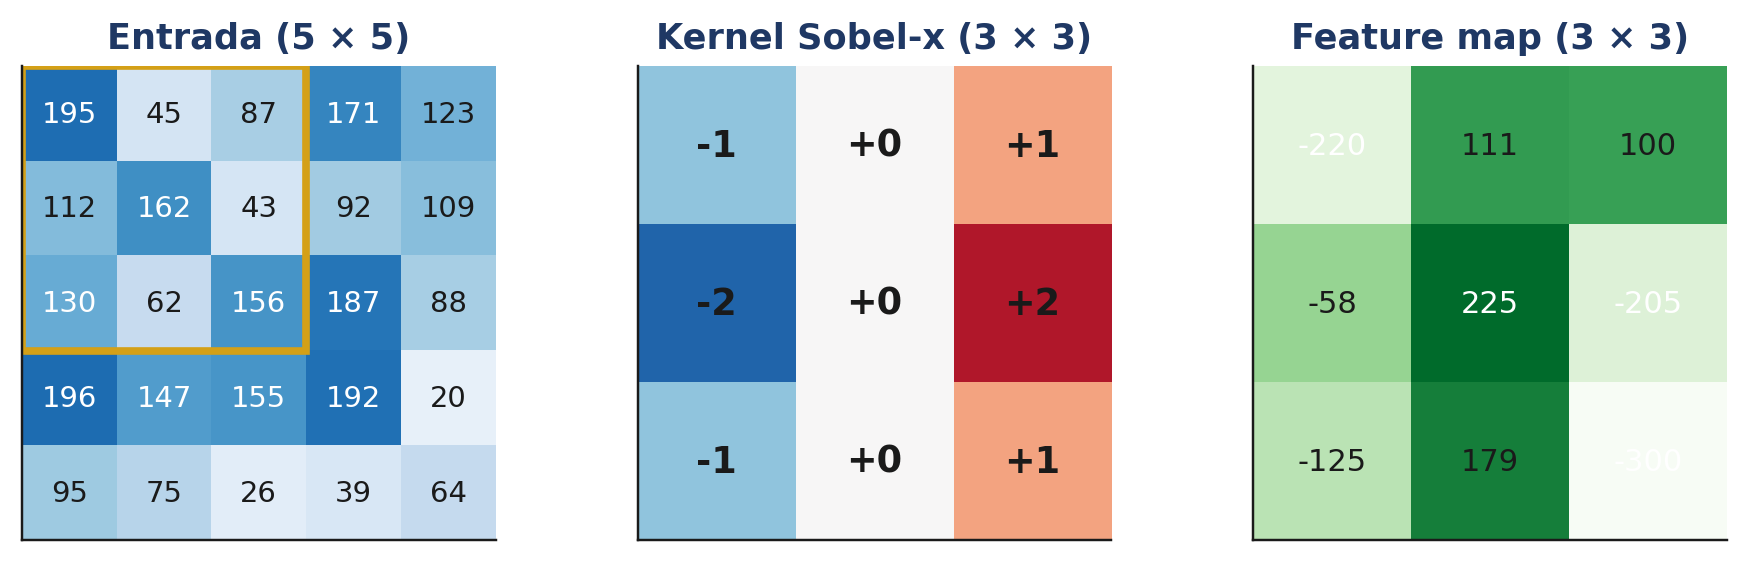
\includegraphics[width=0.8\textwidth]{../docs/assets/g1/g1_fig05_convolution.png}
\caption{Operación de convolución: un filtro recorre la imagen y produce un mapa de características. Fuente: Stanford CS231n.}
\label{fig:conv}
\end{figure}

\begin{figure}[h]
\centering
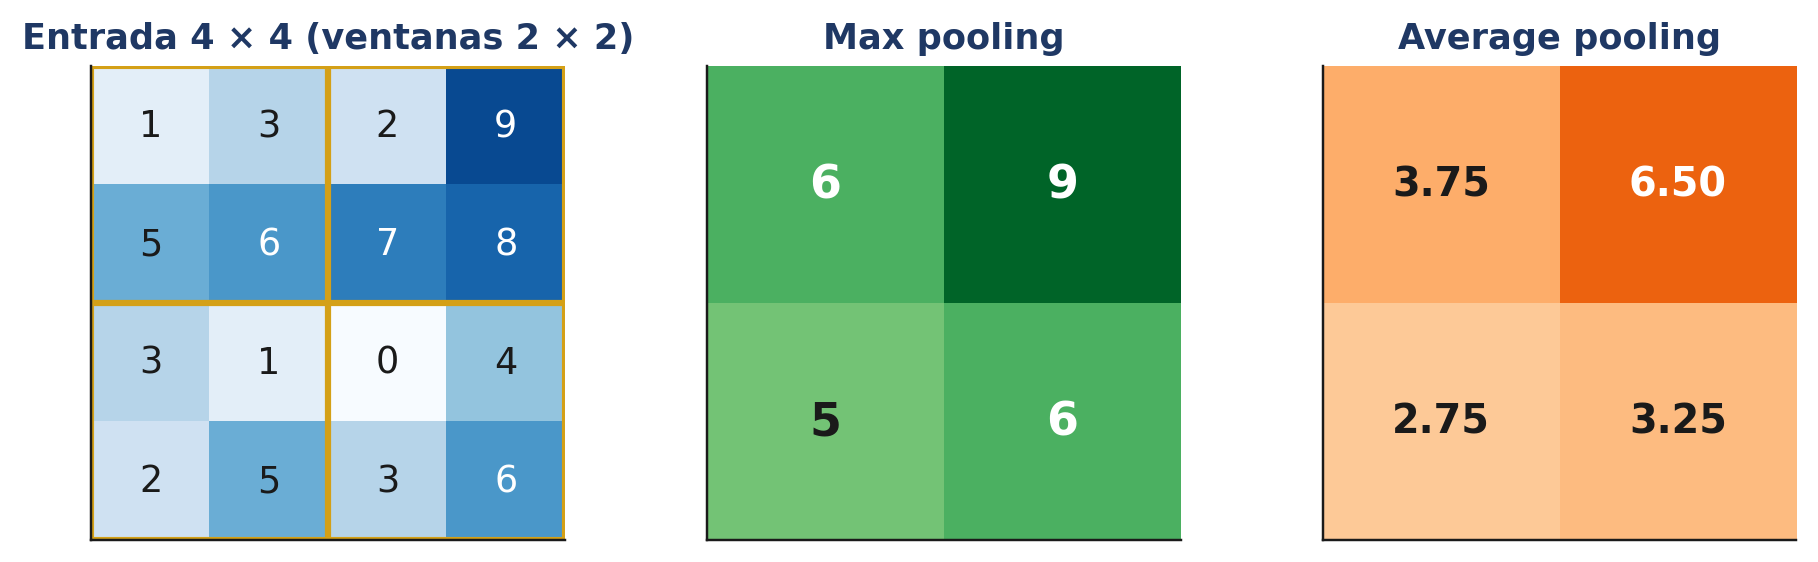
\includegraphics[width=0.78\textwidth]{../docs/assets/g1/g1_fig07_pooling.png}
\caption{Max pooling: cada región se resume por su valor máximo, reduciendo la resolución. Fuente: elaboración propia.}
\label{fig:pool}
\end{figure}

\begin{figure}[h]
\centering
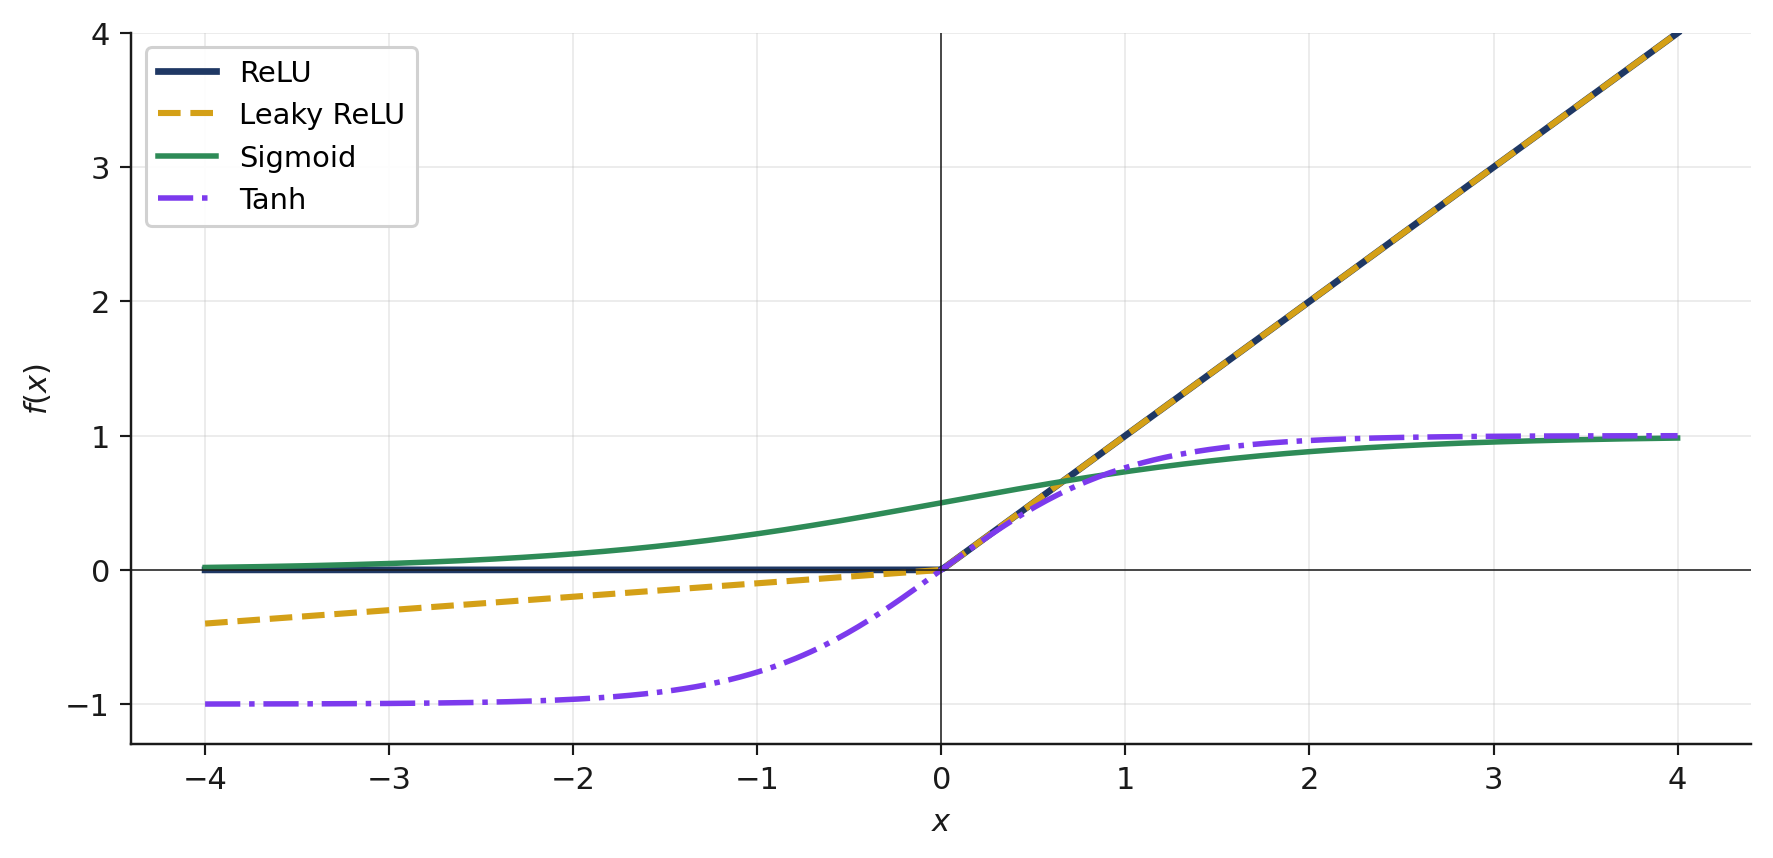
\includegraphics[width=0.78\textwidth]{../docs/assets/g1/g1_fig08_activations.png}
\caption{Funciones de activación habituales. \emph{ReLU} es la más usada en capas convolucionales. Fuente: elaboración propia.}
\label{fig:act}
\end{figure}

\section{Entrenamiento y evaluación}

El entrenamiento ajusta los filtros minimizando una \emph{función de pérdida}
(\emph{categorical crossentropy} para clasificación multiclase) mediante
\emph{backpropagation} y un optimizador (\emph{Adam} por defecto). El proceso se repite
durante varias \emph{épocas} sobre lotes (\emph{batches}) de imágenes.

El desempeño se mide sobre un conjunto de \textbf{validación} independiente. La
\emph{accuracy} y la \textbf{matriz de confusión} revelan no solo cuánto acierta el
modelo, sino dónde se confunde. Si la accuracy en entrenamiento es alta pero la de
validación es baja, el modelo sufre \emph{overfitting}: memoriza en lugar de generalizar.

\section{Aumentación de datos}

La \emph{data augmentation} genera variaciones de las imágenes de entrenamiento
---rotaciones, desplazamientos, cambios de brillo, zoom--- para que el modelo generalice
mejor con pocos datos. Es la primera defensa contra el \emph{overfitting} sin modificar
la arquitectura.

% =============================================================================
\section{Experiencia guiada}\label{sec:guiada}

El trabajo se desarrolla en tres notebooks que la pareja ejecuta y completa. La
indicación es la misma para todos: \textbf{ejecutar el notebook de principio a fin,
completar las celdas marcadas como \emph{«completar»} y responder por escrito las
preguntas conceptuales}. Como los notebooks ya vienen implementados, \textbf{la nota
evalúa la comprensión}: las respuestas a las preguntas conceptuales y la interpretación y
justificación de los resultados, no la simple ejecución. La rúbrica completa está en la
\emph{Ficha de Evaluación}: la Parte~1 aporta \textbf{10 puntos} y la Parte~2 otros 10,
para una nota sobre 20.

Los Notebooks 1 y 2 usan el dataset de botellas (vidrio/plástico) provisto; el Notebook~3
usa un dataset de tapitas construido por la propia pareja. El dataset se organiza en
subcarpetas por clase dentro de \texttt{train/} y \texttt{validation/}, de modo que
\texttt{ImageDataGenerator} infiera las etiquetas automáticamente:

\begin{center}
\begin{tikzpicture}[
  every node/.style={font=\footnotesize\ttfamily},
  level distance=8mm, sibling distance=20mm,
  level 1/.style={sibling distance=40mm}, level 2/.style={sibling distance=18mm},
]
\node {data/botellas/}
  child { node {train/} child { node {vidrio/} } child { node {plastico/} } }
  child { node {validation/} child { node {vidrio/} } child { node {plastico/} } };
\end{tikzpicture}
\end{center}

\subsection{Notebook 1: CNN desde cero}

Recorre el ciclo completo de una CNN entrenada desde cero: carga del dataset, definición
y compilación de la arquitectura (Figura~\ref{fig:arch}: bloques
\texttt{Conv2D}\,+\,\texttt{MaxPooling2D}, \texttt{Flatten}, capa densa con \emph{dropout}
y salida \emph{softmax}), entrenamiento, evaluación con matriz de confusión y predicción
sobre imágenes propias (Figuras~\ref{fig:curvas} y~\ref{fig:confmat}).

\begin{figure}[h]
\centering
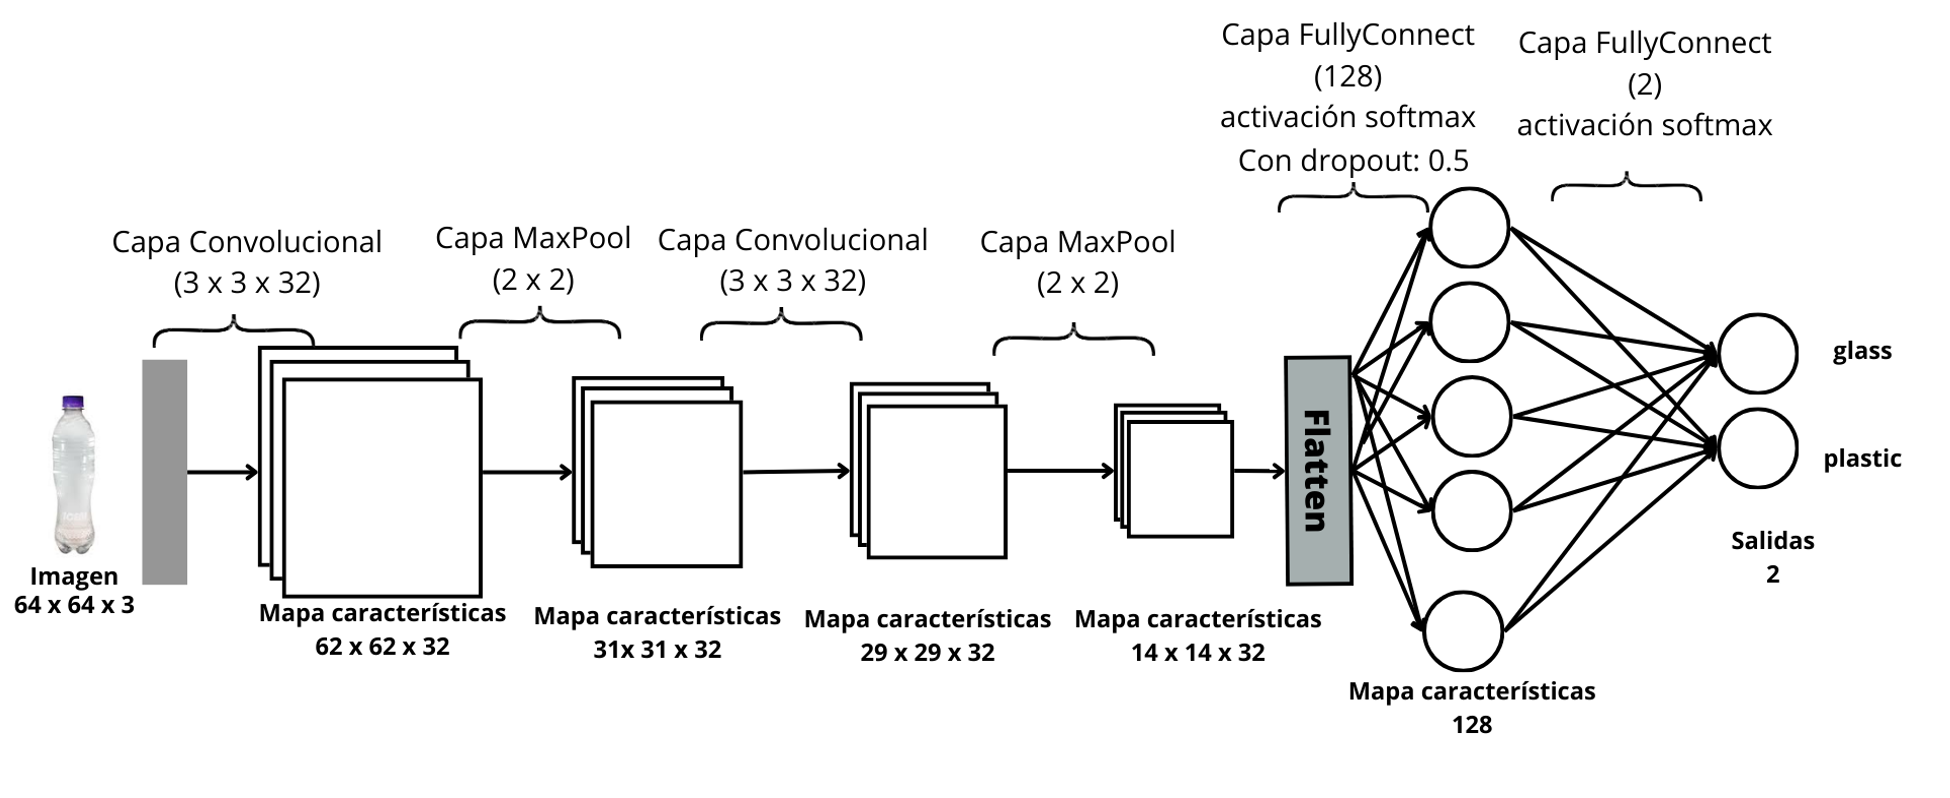
\includegraphics[width=0.95\textwidth]{../docs/assets/g1/arquitectura_botellas.png}
\caption{Arquitectura de la CNN del laboratorio. Fuente: elaboración propia (NN-SVG).}
\label{fig:arch}
\end{figure}

\renewcommand{\arraystretch}{1.3}
\begin{tabularx}{\textwidth}{@{}p{6.2cm} X r@{}}
\toprule
\textbf{Etapa (secciones del notebook)} & \textbf{Qué se realiza} & \textbf{Puntos} \\
\midrule
1. Arquitectura y entrenamiento \newline (secciones 3--6)
  & Definir y compilar la CNN, entrenar y analizar las curvas de \emph{loss}/\emph{accuracy} y la matriz de confusión sobre validación.
  & 1.5 \\
2. Evaluación con datos propios \newline (sección 7)
  & Clasificar cuatro fotografías capturadas por la pareja en condiciones variadas e identificar aciertos y fallos.
  & 1.5 \\
\bottomrule
\end{tabularx}
\renewcommand{\arraystretch}{1}

\begin{figure}[h]
\centering
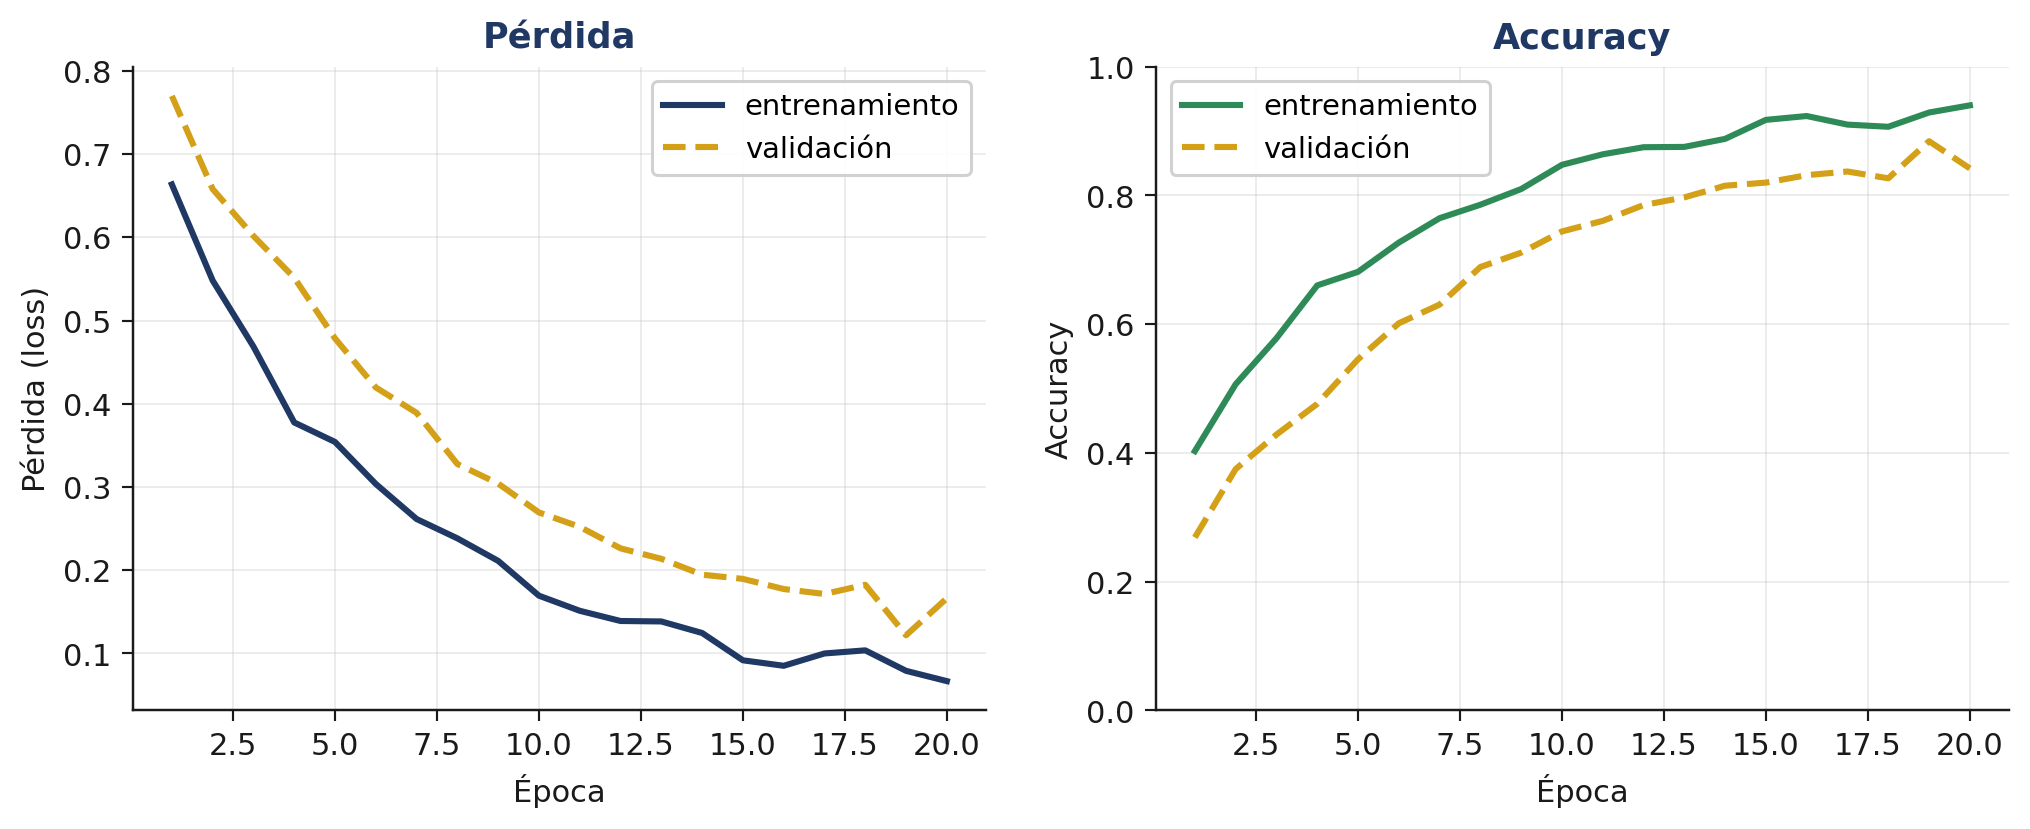
\includegraphics[width=0.82\textwidth]{../docs/assets/g1/g1_fig12_training_curves.png}
\caption{Curvas de aprendizaje esperadas sobre el dataset de botellas. Fuente: elaboración propia.}
\label{fig:curvas}
\end{figure}

\begin{figure}[h]
\centering
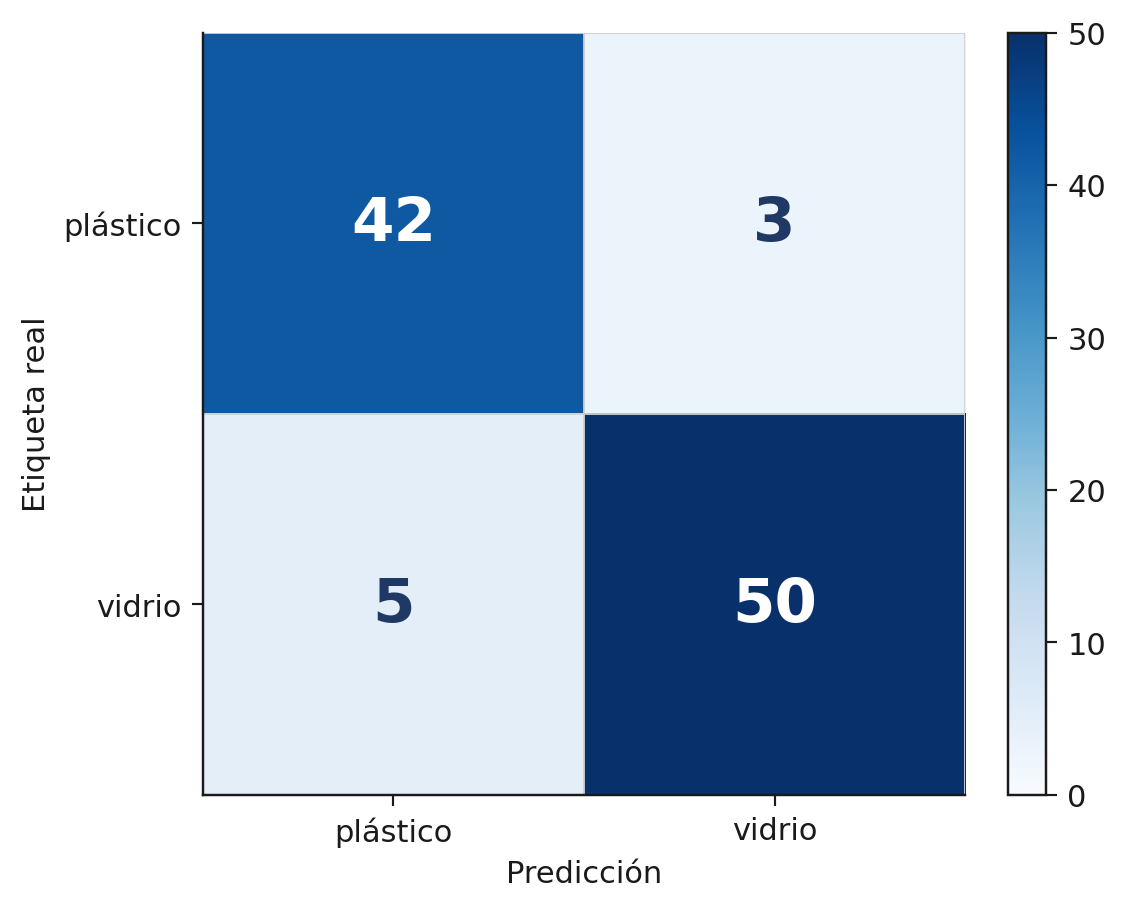
\includegraphics[width=0.45\textwidth]{../docs/assets/g1/g1_fig11_confmat.png}
\caption{Matriz de confusión sobre validación: la diagonal son aciertos. Fuente: elaboración propia.}
\label{fig:confmat}
\end{figure}

\subsection{Notebook 2: aumentación de datos}

Retoma el clasificador anterior para evidenciar y mitigar el \emph{overfitting}: reproduce
el sobreajuste del modelo base, selecciona transformaciones de aumentación pertinentes,
reentrena y compara el desempeño frente al modelo sin aumentar.

\renewcommand{\arraystretch}{1.3}
\begin{tabularx}{\textwidth}{@{}p{6.2cm} X r@{}}
\toprule
\textbf{Etapa (secciones del notebook)} & \textbf{Qué se realiza} & \textbf{Puntos} \\
\midrule
3. Data augmentation \newline (secciones 2--5)
  & Diagnosticar el \emph{overfitting} del modelo base, seleccionar transformaciones justificadas, reentrenar y comparar curvas frente al modelo base.
  & 2.5 \\
\bottomrule
\end{tabularx}
\renewcommand{\arraystretch}{1}

\subsection{Notebook 3: clasificador de tapitas}

Introduce un dataset propio: tapitas de colores (\textbf{rojo}, \textbf{azul},
\textbf{amarillo}) más una clase \texttt{fondo} (imágenes sin tapita). La pareja graba un
video corto por color, el notebook extrae los \emph{frames} a \texttt{data/tapitas/<clase>/}
(descartando los borrosos), divide en \emph{train}/\emph{validation} y entrena una CNN desde
cero. El modelo se exporta a \texttt{modelos/} para reutilizarlo en la Parte~2.

\textbf{Protocolo de captura:} iluminación y fondos variados, distancia 10--40\,cm,
ángulos diversos, una sola tapita por imagen y al menos 50 muestras por clase.

\renewcommand{\arraystretch}{1.3}
\begin{tabularx}{\textwidth}{@{}p{6.2cm} X r@{}}
\toprule
\textbf{Etapa (pasos del notebook)} & \textbf{Qué se realiza} & \textbf{Puntos} \\
\midrule
4. Captura y preparación del dataset \newline (pasos 1--2)
  & Grabar un video por color, extraer los frames a \texttt{data/tapitas/} y reportar el conteo por clase.
  & 1.0 \\
5. Entrenamiento y evaluación CNN \newline (pasos 3--4)
  & Dividir \emph{train}/\emph{validation}, entrenar la CNN, analizar curvas y matriz de confusión, y exportar el modelo.
  & 2.0 \\
\bottomrule
\end{tabularx}
\renewcommand{\arraystretch}{1}

\subsection{Cierre: discusión crítica}

A partir de los resultados, la pareja formula al menos dos hipótesis técnicas sobre las
causas de los errores (sesgos del dataset, sensibilidad a la iluminación, límites de la
arquitectura) y propone dos estrategias de mejora sin cambiar la arquitectura. Se
documenta en la Ficha de Evaluación (\textbf{1.5 puntos}).

\begin{center}
\renewcommand{\arraystretch}{1.3}
\begin{tabular}{@{}lr@{}}
\toprule
\textbf{Distribución de la nota de la Parte 1} & \textbf{Puntos} \\
\midrule
Notebook 1 --- \texttt{notebook1\_cnn\_desde\_cero.ipynb}      & 3.0 \\
Notebook 2 --- \texttt{notebook2\_data\_augmentation.ipynb}    & 2.5 \\
Notebook 3 --- \texttt{notebook3\_clasificador\_tapitas.ipynb} & 3.0 \\
Discusión crítica                                              & 1.5 \\
\midrule
\textbf{Total Parte 1} & \textbf{10.0} \\
\bottomrule
\end{tabular}
\renewcommand{\arraystretch}{1}
\end{center}

% =============================================================================
\section{Cierre: el límite del entrenamiento desde cero}\label{sec:cierre}

La evaluación sobre datos propios suele revelar un resultado aleccionador: el modelo
alcanza buena \emph{accuracy} en validación, pero \textbf{falla ante condiciones reales}
de iluminación, fondo o ángulo distintas a las del entrenamiento. La aumentación
(Notebook~2) mitiga el problema pero no lo resuelve: una CNN entrenada desde cero necesita
muchas más imágenes de las que es razonable capturar a mano.

Ese es el límite que motiva la \textbf{Parte 2}: en lugar de aprender todos los filtros
desde cero, se parte de una red ya entrenada sobre millones de imágenes y se reutiliza su
conocimiento ---\emph{aprendizaje por transferencia}---, obteniendo clasificadores robustos
con apenas unos cientos de imágenes por clase. Sobre esa técnica se construye el sistema de
control de calidad de la segunda parte, reutilizando el dataset de tapitas del Notebook~3.


\clearpage
\part{Visión por Computadora: Transfer Learning y Beckhoff}
\section{Introducción}

Esta es la \textbf{Parte~2} del laboratorio: visión por computadora aplicada al control de
calidad. Se reutiliza el dataset de tapitas de la Parte~1, pero ahora el modelo se entrena
con \emph{aprendizaje por transferencia} (MobileNetV2) y el resultado se envía a un IPC
\textbf{Beckhoff} por el protocolo \textbf{ADS} para accionar un brazo robótico.

\textbf{Materiales.} Los notebooks \texttt{notebook4\_transfer\_learning.ipynb},
\texttt{notebook5\_probar\_modelo.ipynb} y \texttt{notebook6\_envio\_beckhoff.ipynb}; la
librería \texttt{pyads}; y un proyecto TwinCAT con el IPC Beckhoff.

\section{Aprendizaje por transferencia}\label{sec:tl-concepto}

En lugar de entrenar una red desde cero, el \emph{transfer learning} parte de un modelo ya
entrenado sobre millones de imágenes (\textbf{MobileNetV2}, sobre ImageNet) y reutiliza los
filtros que este aprendió. Se procede en dos fases (Figura~\ref{fig:transfer}):

\begin{itemize}
  \item \textbf{Feature extraction}: se \emph{congela} el \emph{backbone} preentrenado y se
        entrena solo un cabezal nuevo (capa densa \emph{softmax}) para las clases del
        problema. Pocas épocas bastan.
  \item \textbf{Fine-tuning}: se \emph{descongelan} las últimas capas del \emph{backbone} y
        se reentrena con un \emph{learning rate} pequeño, para afinar las características de
        alto nivel al dominio de las tapitas sin destruir lo aprendido.
\end{itemize}

La ventaja es decisiva: se obtienen clasificadores robustos con apenas unos cientos de
imágenes por clase, donde una CNN desde cero necesitaría miles.

\begin{figure}[h]
\centering
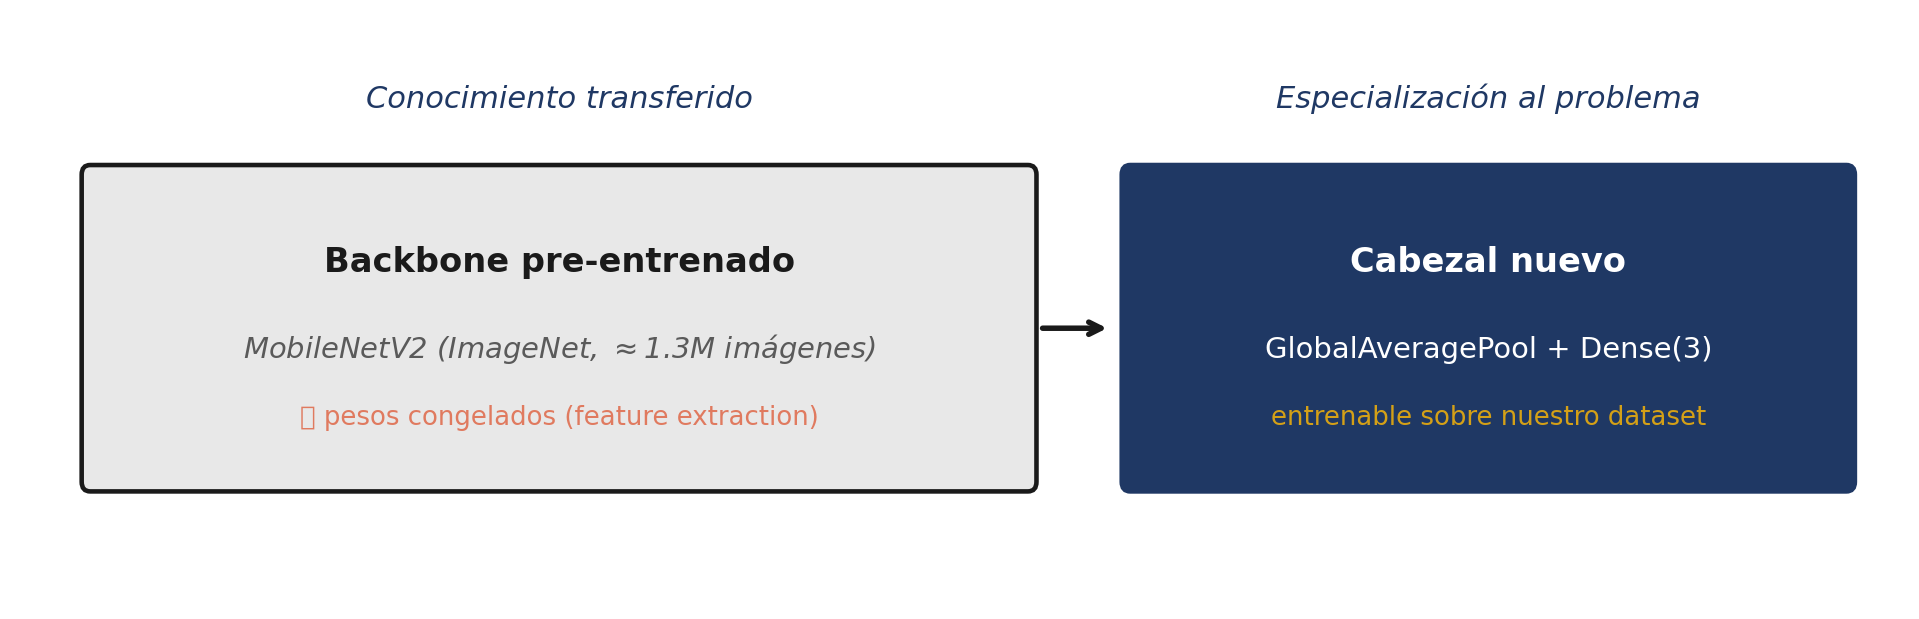
\includegraphics[width=0.95\textwidth]{../docs/assets/g2/transfer_learning.png}
\caption{Aprendizaje por transferencia: se reutiliza el \emph{backbone} preentrenado y se sustituye el clasificador final. Fuente: elaboración propia.}
\label{fig:transfer}
\end{figure}

\section{El dataset de tapitas}

Se reutiliza el dataset construido en la Parte~1 (Notebook~3): cuatro clases en orden
alfabético ---\texttt{amarillo}, \texttt{azul}, \texttt{fondo}, \texttt{rojo}---, con la
división 80\,\% entrenamiento / 20\,\% validación. La clase \texttt{fondo} (imágenes sin
tapita) es defensiva: evita que el modelo fuerce un color cuando no hay objeto y
\textbf{no activa ninguna salida} del PLC. Si el dataset resultó escaso, conviene ampliarlo
con más variación de iluminación, fondo y ángulo.

% =============================================================================
\section{Protocolo ADS y comunicación con Beckhoff}

El \textbf{ADS} (\emph{Automation Device Specification}) es el protocolo de Beckhoff para
intercambiar datos con el runtime TwinCAT. Permite acceder a las variables del PLC por su
\textbf{nombre simbólico} (dentro de una \emph{Global Variable List}, GVL), sobre TCP/IP y
desde cualquier lenguaje; desde Python se usa la librería \texttt{pyads}
(Figura~\ref{fig:ads}).

\begin{figure}[h]
\centering
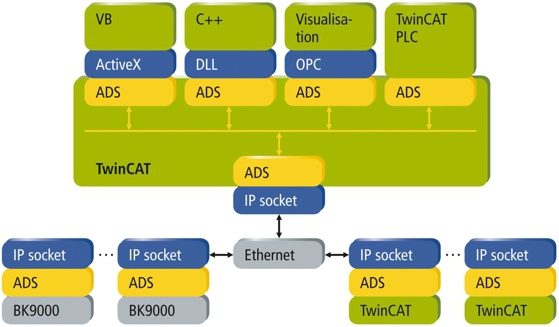
\includegraphics[width=0.8\textwidth]{../docs/assets/g2/ads_protocol.png}
\caption{Arquitectura del protocolo ADS: las aplicaciones cliente acceden a las variables del PLC a través del \emph{router} de TwinCAT. Fuente: Beckhoff Automation.}
\label{fig:ads}
\end{figure}

\subsection{Configuración previa en TwinCAT}

Para que Python pueda escribir en el IPC, del lado TwinCAT se debe:

\begin{enumerate}
  \item Declarar en una GVL llamada \texttt{VARIABLES} tres variables \texttt{BOOL}:
        \texttt{bRojo}, \texttt{bAzul}, \texttt{bAmarillo}.
  \item Configurar una \emph{route} ADS entre la PC y el IPC (AMS Net ID y puerto 851).
  \item Construir un \textbf{HMI} en TwinCAT con una \textbf{lámpara por color}, cada una
        enlazada a su variable \texttt{BOOL}, para verificar visualmente que el clasificador
        escribe la variable correcta.
\end{enumerate}

\subsection{La librería \texttt{pyads}}

El patrón básico de conexión y escritura se muestra en el Script~\ref{lst:pyads-basic}.
Los nombres en \texttt{write\_by\_name()} deben coincidir \emph{exactamente} con los de la
GVL (mayúsculas incluidas).

\begin{lstlisting}[language=Python, caption={Conexión y escritura básica con pyads.}, label={lst:pyads-basic}]
import pyads

ipc = pyads.Connection('192.168.57.231.1.1', 851)   # AMS Net ID del IPC
ipc.open()

ipc.write_by_name('VARIABLES.bRojo',     True,  pyads.PLCTYPE_BOOL)
ipc.write_by_name('VARIABLES.bAzul',     False, pyads.PLCTYPE_BOOL)
ipc.write_by_name('VARIABLES.bAmarillo', False, pyads.PLCTYPE_BOOL)

ipc.close()
\end{lstlisting}

% =============================================================================
\section{Integración: del clasificador a la acción del brazo}

El sistema opera bajo un contrato simple: el clasificador procesa el \emph{frame} de la
cámara y, si la confianza supera un umbral configurable (por defecto $0.6$), escribe
\texttt{True} en la variable del color predicho y \texttt{False} en las otras dos; si la
clase es \texttt{fondo} o la confianza es baja, las tres quedan en \texttt{False}. El PLC
detecta el flanco ascendente, activa la salida digital correspondiente y el brazo deposita
la tapita en su zona. El Script~\ref{lst:loop} integra captura, predicción y escritura ADS.

\begin{lstlisting}[language=Python, caption={Bucle principal: captura, predicción y escritura ADS.}, label={lst:loop}]
import cv2, numpy as np, pyads
from tensorflow.keras.models import load_model
from tensorflow.keras.applications.mobilenet_v2 import preprocess_input

UMBRAL = 0.6
IMG_SIZE = 128                                    # igual que al entrenar (NB4)
CLASES = ['amarillo', 'azul', 'fondo', 'rojo']    # orden alfabetico
VAR_POR_CLASE = {                                 # 'fondo' no activa ninguna salida
    'rojo': 'VARIABLES.bRojo',
    'azul': 'VARIABLES.bAzul',
    'amarillo': 'VARIABLES.bAmarillo',
}

modelo = load_model('modelo_tapitas.h5')
ipc = pyads.Connection('192.168.57.231.1.1', 851)
ipc.open()

cam = cv2.VideoCapture(0)
try:
    while True:
        ok, frame = cam.read()
        if not ok:
            break
        # Preprocesamiento MobileNetV2: BGR->RGB, resize y normalizar a [-1, 1]
        img = cv2.cvtColor(cv2.resize(frame, (IMG_SIZE, IMG_SIZE)), cv2.COLOR_BGR2RGB)
        x = np.expand_dims(preprocess_input(img.astype('float32')), axis=0)

        pred = modelo.predict(x, verbose=0)[0]
        idx = int(np.argmax(pred))
        clase, confianza = CLASES[idx], float(pred[idx])

        # Activa el BOOL del color detectado si supera el umbral; el resto en False.
        activo = VAR_POR_CLASE.get(clase) if confianza >= UMBRAL else None
        for var in VAR_POR_CLASE.values():
            ipc.write_by_name(var, var == activo, pyads.PLCTYPE_BOOL)

        cv2.putText(frame, f"{clase} ({confianza:.2f})", (10, 30),
                    cv2.FONT_HERSHEY_SIMPLEX, 0.8, (0, 255, 0), 2)
        cv2.imshow('Clasificador', frame)
        if cv2.waitKey(1) & 0xFF == ord('q'):
            break
finally:
    cam.release(); cv2.destroyAllWindows()
    for var in VAR_POR_CLASE.values():            # apagar todo al salir
        ipc.write_by_name(var, False, pyads.PLCTYPE_BOOL)
    ipc.close()
\end{lstlisting}

% =============================================================================
\section{Experiencia guiada}\label{sec:tl-practico}

La pareja ejecuta y completa los tres notebooks de la Parte~2 (igual que en la Parte~1:
ejecutar de principio a fin, completar las celdas marcadas y responder las preguntas). La
Parte~2 aporta \textbf{10 puntos}.

\renewcommand{\arraystretch}{1.35}
\begin{tabularx}{\textwidth}{@{}p{5.3cm} X r@{}}
\toprule
\textbf{Actividad (herramienta)} & \textbf{Qué se realiza} & \textbf{Puntos} \\
\midrule
1. Feature extraction \newline {\footnotesize(\texttt{notebook4}, secc. 2--6)}
  & Reutilizar el dataset de la Parte~1, construir el modelo con \emph{backbone} MobileNetV2 congelado, entrenar el cabezal y evaluar con curvas y matriz de confusión.
  & 3.0 \\
2. Fine-tuning \newline {\footnotesize(\texttt{notebook4}, secc. 4--5)}
  & Descongelar los últimos \emph{layers}, reentrenar con \emph{learning rate} pequeño y comparar contra la fase anterior y contra la CNN del Notebook~3.
  & 2.0 \\
3. Conexión ADS y HMI \newline {\footnotesize(TwinCAT + \texttt{pyads})}
  & Declarar las tres BOOL en la GVL, construir el HMI con una lámpara por color y escribirlas desde Python (Script~\ref{lst:pyads-basic}), verificando el encendido.
  & 2.0 \\
4. Demostración integrada \newline {\footnotesize(\texttt{notebook6} + brazo)}
  & Ejecutar el bucle de inferencia (Script~\ref{lst:loop}) con la cámara: cada color detectado activa su BOOL y dispara la acción del brazo. Grabar un video.
  & 2.5 \\
5. Discusión final
  & Reflexionar sobre cómo aplicar el sistema en el proyecto integrador de automatización.
  & 0.5 \\
\midrule
\textbf{Total Parte 2} & & \textbf{10.0} \\
\bottomrule
\end{tabularx}
\renewcommand{\arraystretch}{1}

% =============================================================================
\section{Anexos}

\subsection*{Anexo B1. Variables del proyecto TwinCAT}

\renewcommand{\arraystretch}{1.2}
\begin{tabularx}{\textwidth}{@{}p{3.0cm} p{2.0cm} X@{}}
\toprule
\textbf{Variable} & \textbf{Tipo} & \textbf{Descripción} \\
\midrule
\texttt{bRojo}     & \texttt{BOOL} & Verdadero al detectar una tapita roja sobre el umbral. \\
\texttt{bAzul}     & \texttt{BOOL} & Verdadero al detectar una tapita azul sobre el umbral. \\
\texttt{bAmarillo} & \texttt{BOOL} & Verdadero al detectar una tapita amarilla sobre el umbral. \\
\bottomrule
\end{tabularx}
\renewcommand{\arraystretch}{1}

Deben declararse dentro de la GVL \texttt{VARIABLES}; el nombre de la GVL forma parte del
identificador usado en \texttt{write\_by\_name()}.

\subsection*{Anexo B2. Diagnóstico de errores comunes}

\renewcommand{\arraystretch}{1.2}
\begin{tabularx}{\textwidth}{@{}p{5.5cm} X@{}}
\toprule
\textbf{Error} & \textbf{Causa y solución} \\
\midrule
\texttt{Missing ADS routes (7)} & Falta la \emph{route} ADS entre la PC y el IPC (\texttt{open()} no la valida; el error aparece al leer/escribir). Crearla en TwinCAT (bandeja) $\rightarrow$ Router $\rightarrow$ Edit Routes $\rightarrow$ Add Route. \\
\texttt{AdsError: symbol not found} & El nombre en \texttt{write\_by\_name} no coincide con la GVL. Verificar mayúsculas y el prefijo \texttt{VARIABLES.} \\
El brazo no se dispara & La variable se escribe pero el POU del PLC no actúa sobre ella. Verificar la lógica en TwinCAT. \\
Confianza alta pero clase incorrecta & Dataset poco diverso. Capturar más muestras en condiciones variadas. \\
\bottomrule
\end{tabularx}
\renewcommand{\arraystretch}{1}


\end{document}
